\chapter{Resultados}
Neste capítulo serão descritos os resultados obtidos através da simulação da
EDP com a variação de diversos parâmetros. Os parâmetros iniciais escolhidos
para este trabalho foram:
\begin{itemize}
    \item $L_x = 10$m (comprimento do domínio)
    \item $nx = 200$ (número de células)
    \item $\bar{u} = 2$m/s (velocidade de escoamento)
    \item $t_\text{final} = 1$s  (tempo final de simulação)
    \item $\Delta x = \frac{L_x}{nx} = 0,05$m (passo no espaço)
    \item $\Delta t = 0,9\left( \frac{\Delta_x}{\bar{u}} \right) = 0,0225$s
          (passo de tempo)
    \item $A = 100$
    \item $B = 1,5$
    \item $C = 4,0$
    \item $D = 6,0$
    \item $E = 2,0$
\end{itemize}

\section{Forward Time-Backward Space (FTBS)}

\subsection{Resultados para variações de $nx$}
Com a variação de $nx$, obtiveram-se os seguintes resultados:
\begin{figure}[H]
    \centering
    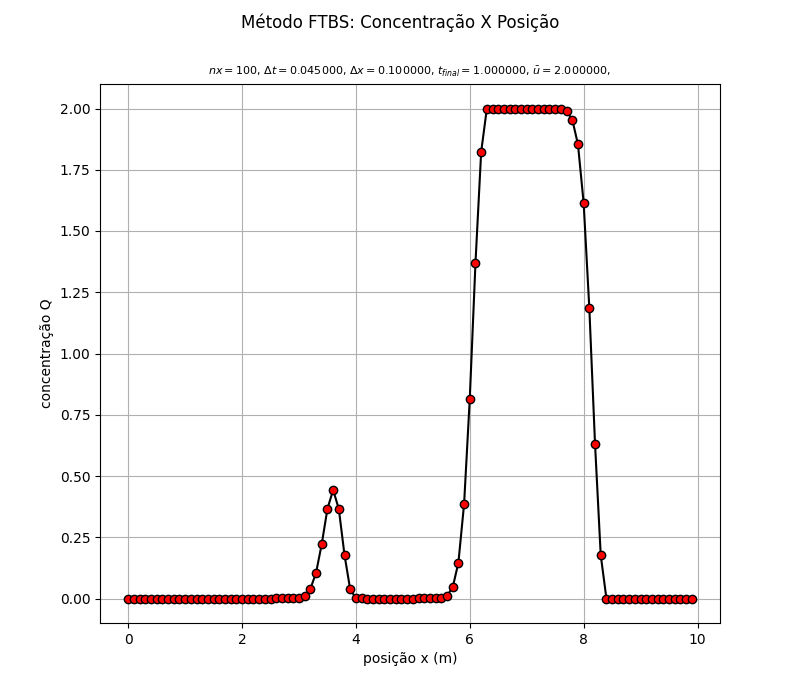
\includegraphics[width=0.7\textwidth]{FTBSnx100}
    \caption{FTBS: $nx = 100$}
\end{figure}
\begin{figure}[H]
    \centering
    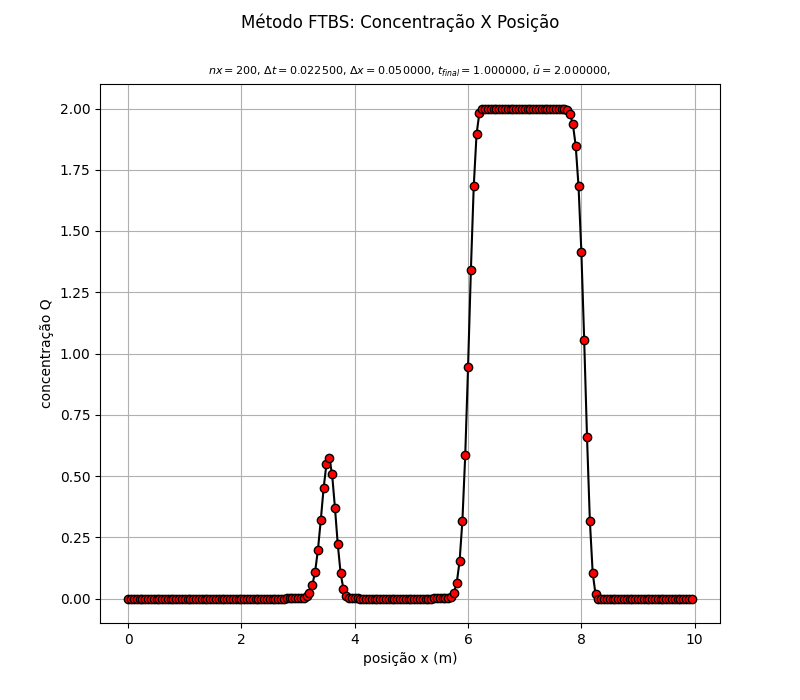
\includegraphics[width=0.7\textwidth]{FTBSnx200}
    \caption{FTBS: $nx = 200$}
\end{figure}
\begin{figure}[H]
    \centering
    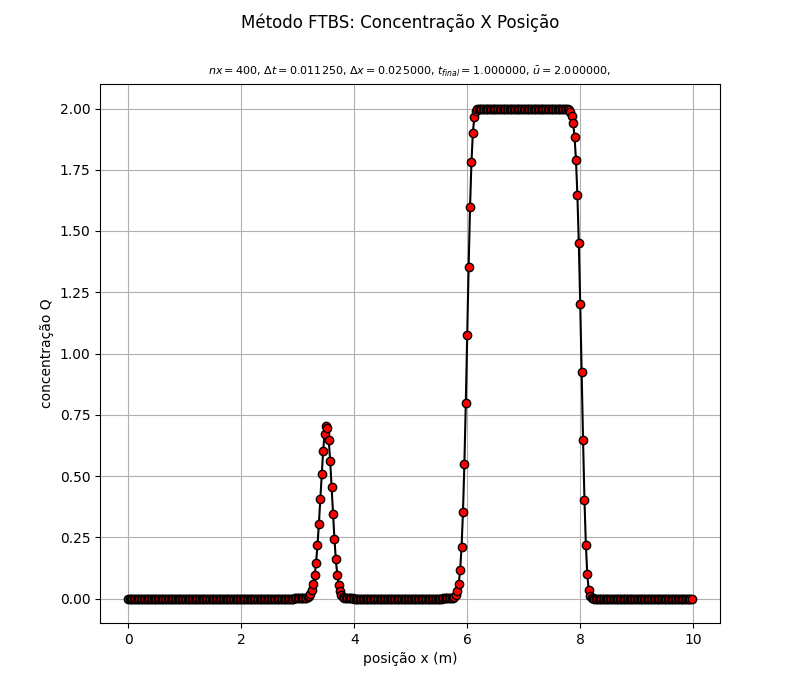
\includegraphics[width=0.7\textwidth]{FTBSnx400}
    \caption{FTBS: $nx = 400$}
\end{figure}
Nota-se que o refinamento da malha resulta em uma curva mais suave, devido ao
aumento da resolução. Este aumento no número de nós torna a solução discreta
mais próxima da contínua (solução real).

\subsection{Resultados para variações de $t_{\text{final}}$}
Com a variação de $t_{\text{final}}$, obtiveram-se os seguintes resultados:
\begin{figure}[H]
    \centering
    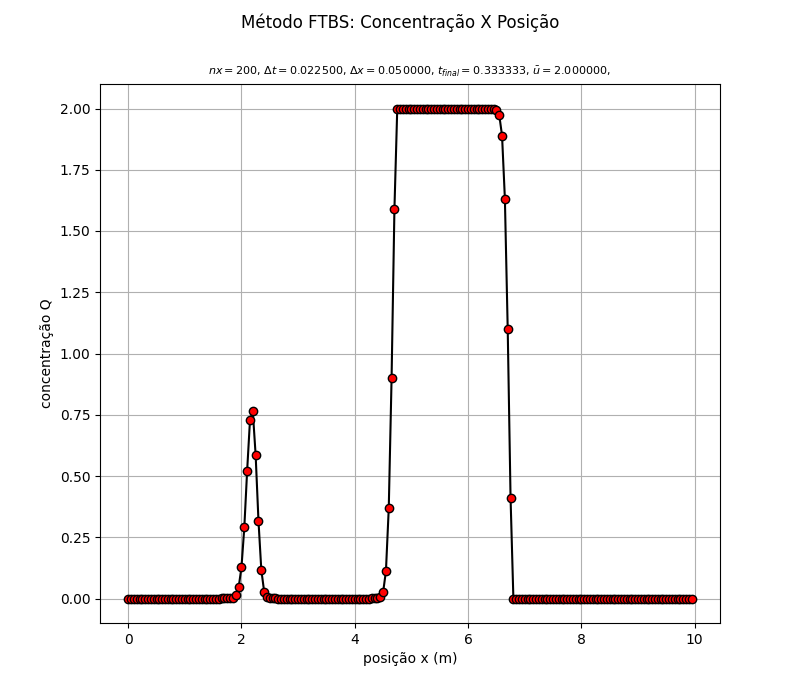
\includegraphics[width=0.7\textwidth]{FTBSt_final0,333}
    \caption{FTBS: $t_{\text{final}} = \frac{1}{3}$s}
\end{figure}
\begin{figure}[H]
    \centering
    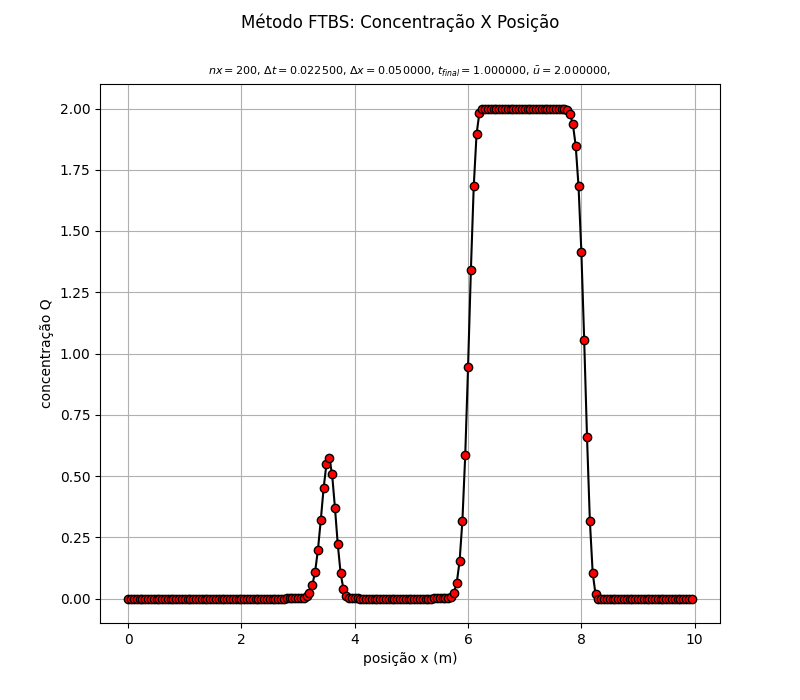
\includegraphics[width=0.7\textwidth]{FTBSt_final1,0}
    \caption{FTBS: $t_{\text{final}} = 1,0$s}
\end{figure}
\begin{figure}[H]
    \centering
    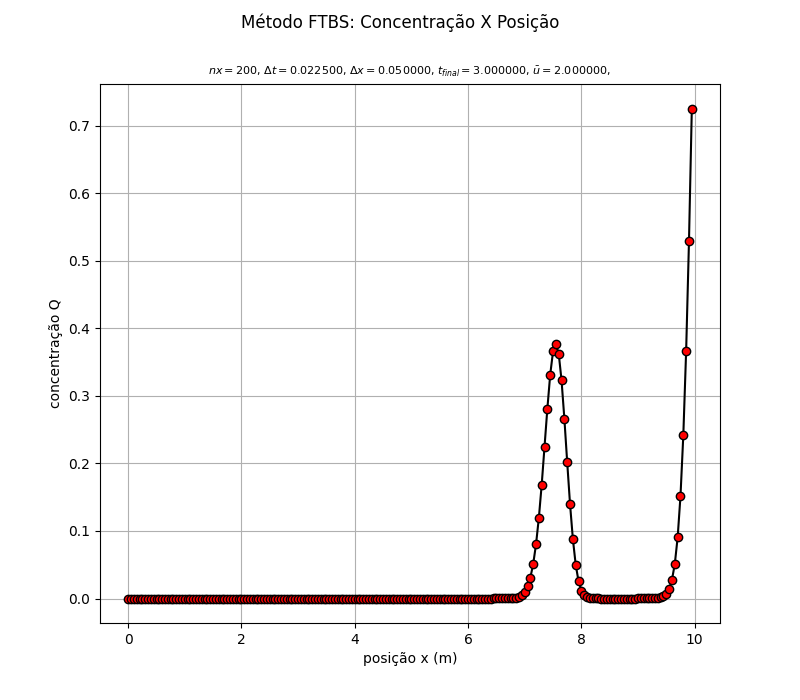
\includegraphics[width=0.7\textwidth]{FTBSt_final3,0}
    \caption{FTBS: $t_{\text{final}} = 3,0$s}
\end{figure}
\begin{figure}[H]
    \centering
    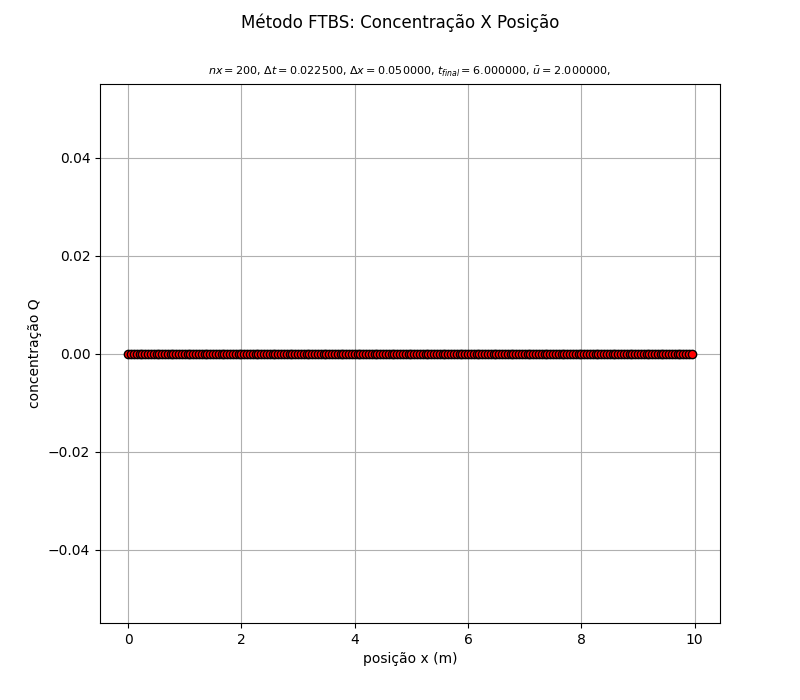
\includegraphics[width=0.7\textwidth]{FTBSt_final6,0}
    \caption{FTBS: $t_{\text{final}} = 6,0$s}
\end{figure}
Nota-se com o avanço do tempo, a onda, representada no gráfico, tende a se
deslocar para a direita, devido ao valor de $\bar{u}$ positivo. Para um tempo
grande o suficiente, a concentração se estabiliza em zero.

\section{Lax-Friedrichs (L-F)}

\subsection{Resultados para variações de $nx$}
Com a variação de $nx$, obtiveram-se os seguintes resultados:
\begin{figure}[H]
    \centering
    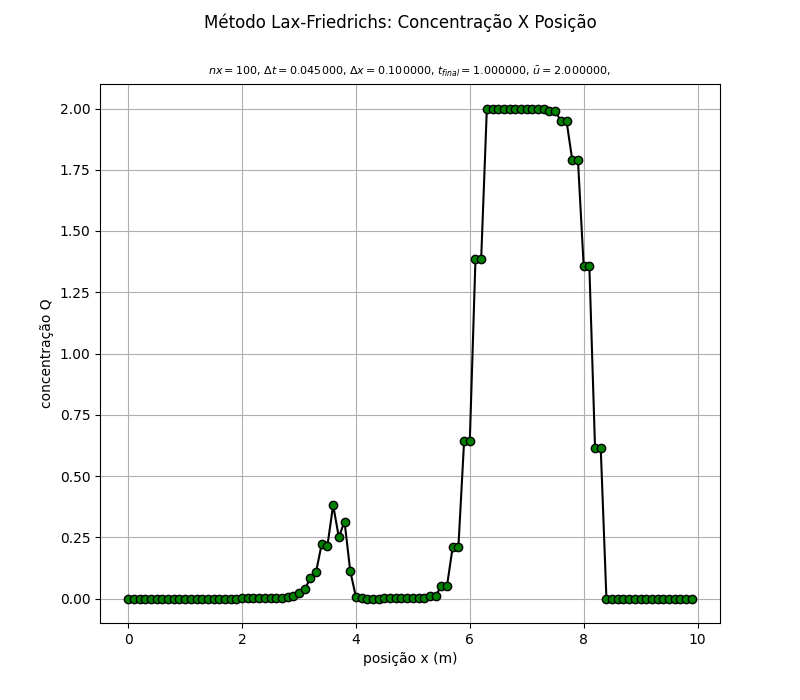
\includegraphics[width=0.7\textwidth]{LFnx100}
    \caption{L-F: $nx = 100$}
\end{figure}
\begin{figure}[H]
    \centering
    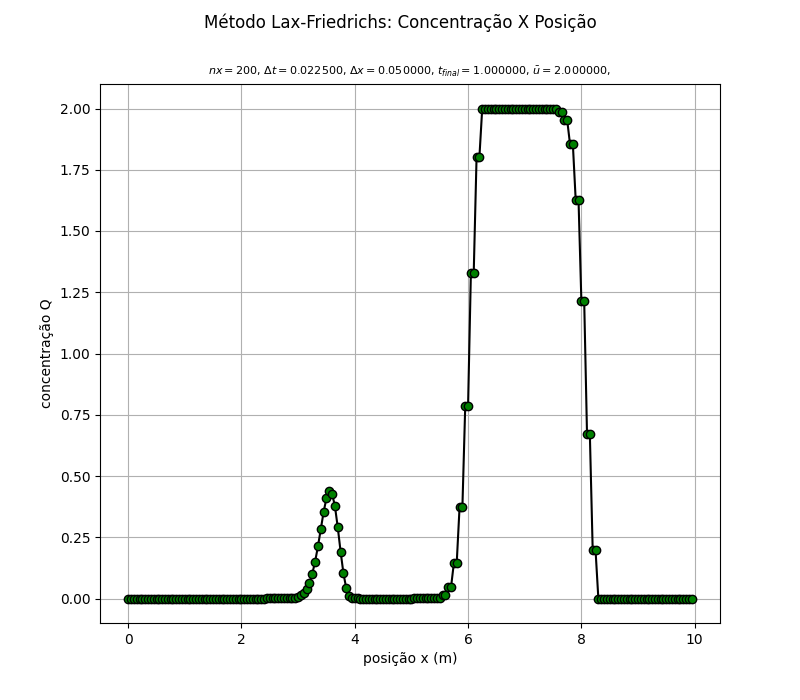
\includegraphics[width=0.7\textwidth]{LFnx200}
    \caption{L-F: $nx = 200$}
\end{figure}
\begin{figure}[H]
    \centering
    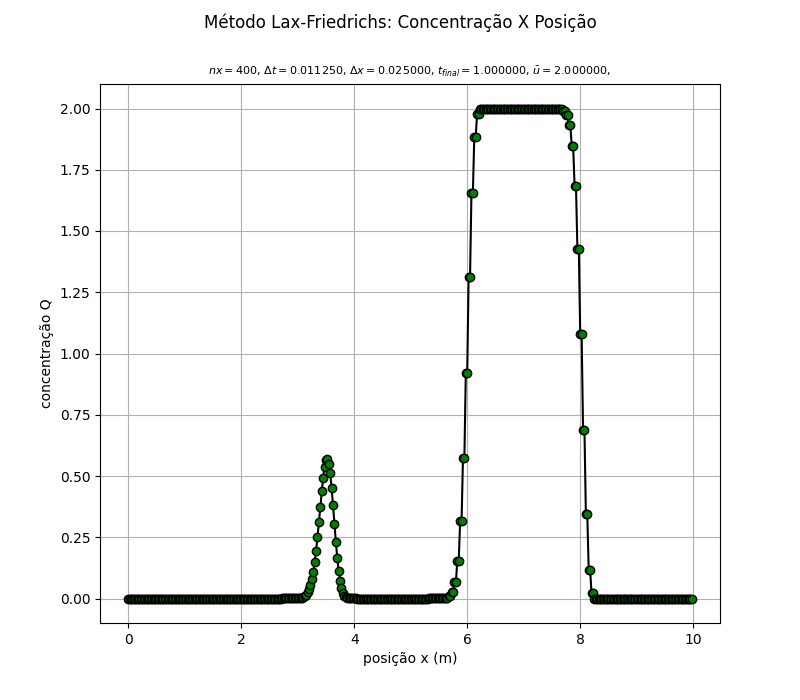
\includegraphics[width=0.7\textwidth]{LFnx400}
    \caption{L-F: $nx = 400$}
\end{figure}
Nota-se que o refinamento da malha resulta em uma curva mais suave, devido ao
aumento da resolução. Este aumento no número de nós torna a solução discreta
mais próxima da contínua (solução real).

\subsection{Resultados para variações de $t_{\text{final}}$}
Com a variação de $t_{\text{final}}$, obtiveram-se os seguintes resultados:
\begin{figure}[H]
    \centering
    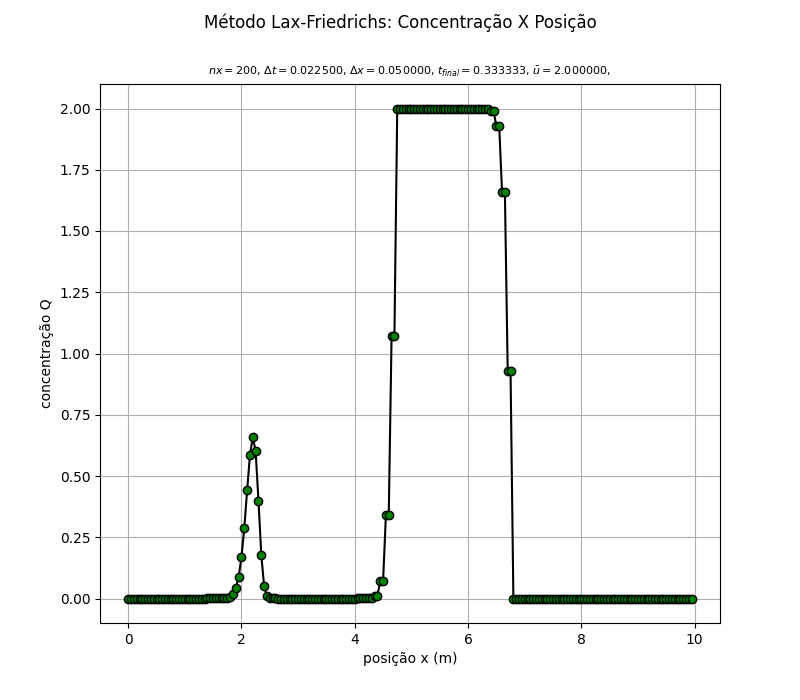
\includegraphics[width=0.7\textwidth]{LFt_final0,333}
    \caption{L-F: $t_{\text{final}} = \frac{1}{3}$s}
\end{figure}
\begin{figure}[H]
    \centering
    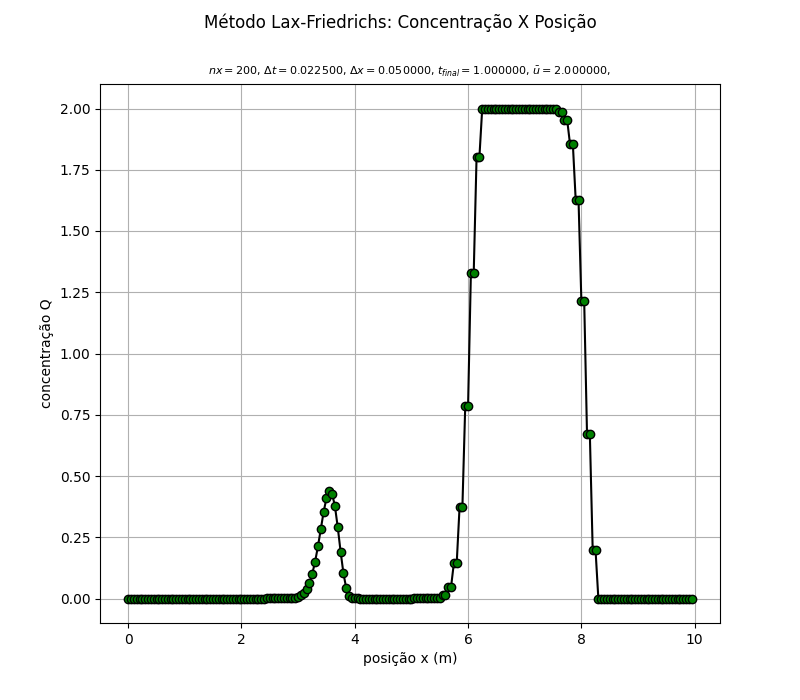
\includegraphics[width=0.7\textwidth]{LFt_final1,0}
    \caption{L-F: $t_{\text{final}} = 1,0$s}
\end{figure}
\begin{figure}[H]
    \centering
    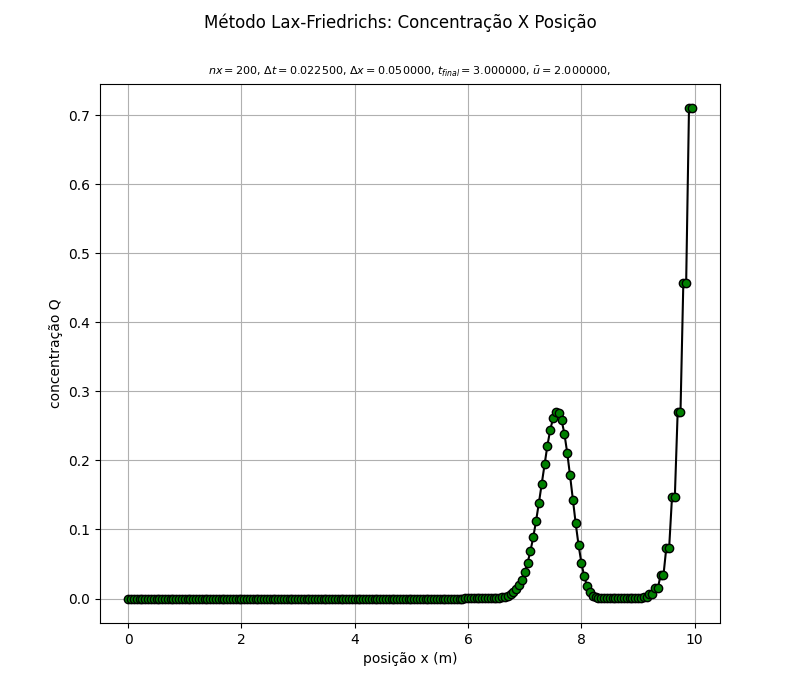
\includegraphics[width=0.7\textwidth]{LFt_final3,0}
    \caption{L-F: $t_{\text{final}} = 3,0$s}
\end{figure}
\begin{figure}[H]
    \centering
    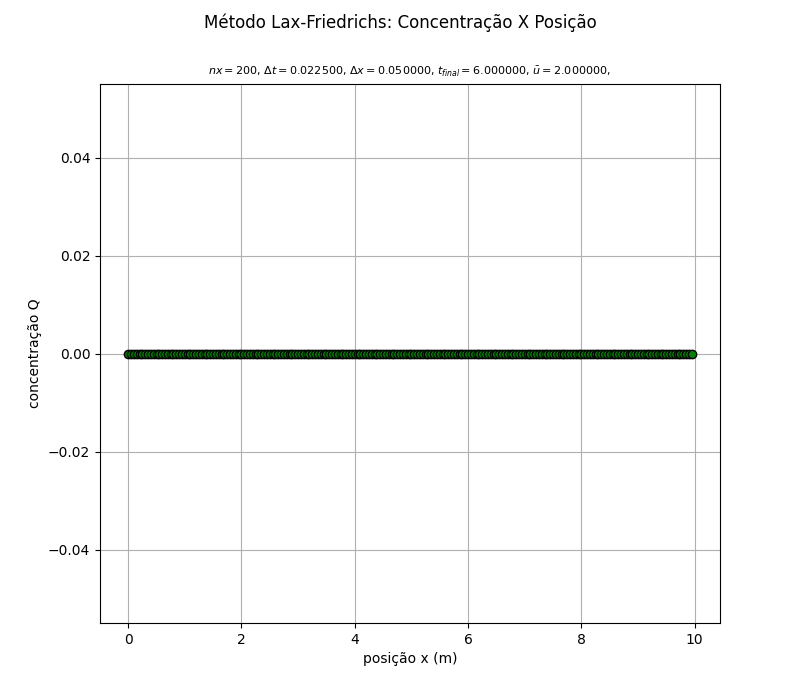
\includegraphics[width=0.7\textwidth]{LFt_final6,0}
    \caption{L-F: $t_{\text{final}} = 6,0$s}
\end{figure}
Nota-se com o avanço do tempo, a onda, representada no gráfico, tende a se
deslocar para a direita, devido ao valor de $\bar{u}$ positivo. Para um tempo
grande o suficiente, a concentração se estabiliza em zero.

\section{Lax-Wendroff (L-W)}

\subsection{Resultados para variações de $nx$}
Com a variação de $nx$, obtiveram-se os seguintes resultados:
\begin{figure}[H]
    \centering
    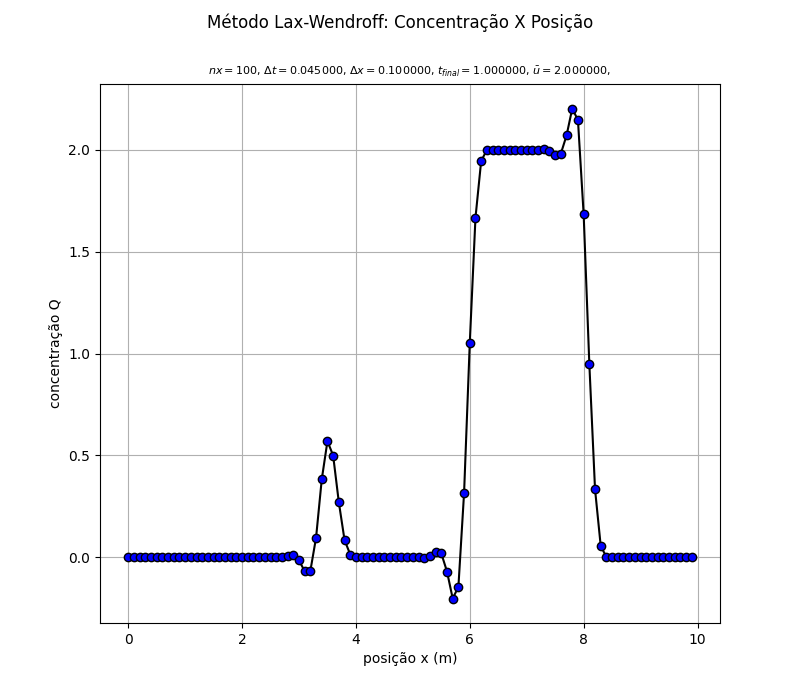
\includegraphics[width=0.7\textwidth]{LWnx100}
    \caption{L-W: $nx = 100$}
\end{figure}
\begin{figure}[H]
    \centering
    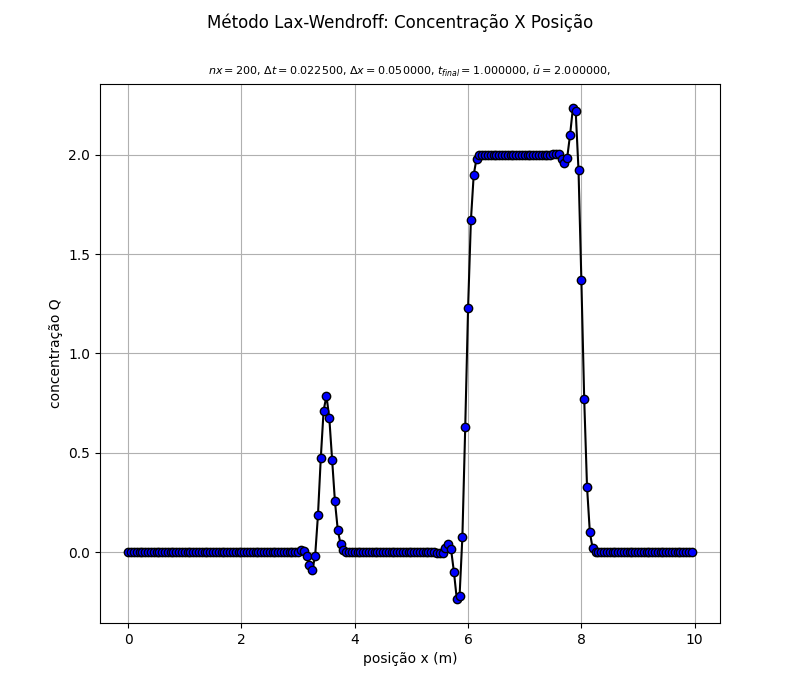
\includegraphics[width=0.7\textwidth]{LWnx200}
    \caption{L-W: $nx = 200$}
\end{figure}
\begin{figure}[H]
    \centering
    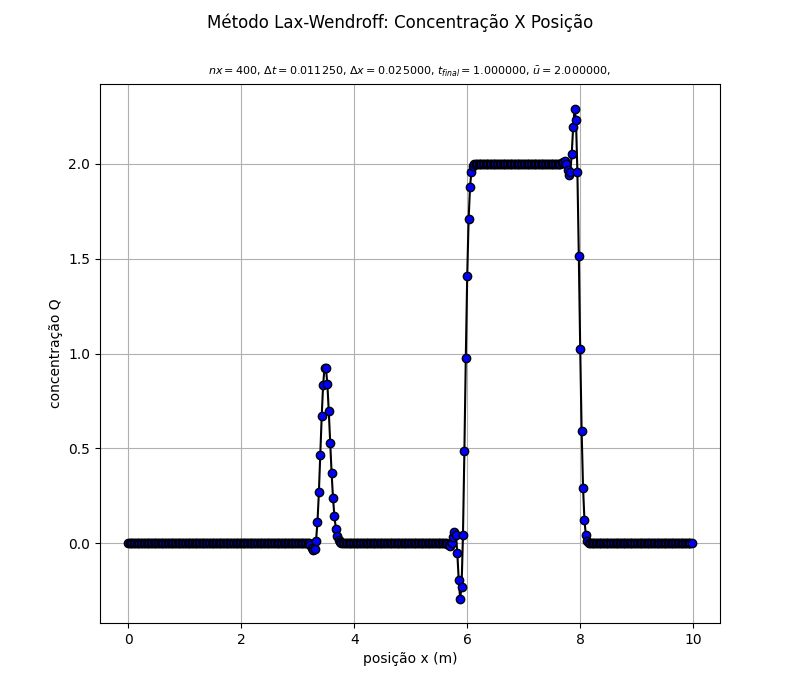
\includegraphics[width=0.7\textwidth]{LWnx400}
    \caption{L-W: $nx = 400$}
\end{figure}
Nota-se, com o refinamento da malha, a presença das oscilações numéricas
características do método.

Nota-se que o refinamento da malha resulta em uma curva mais suave, devido ao
aumento da resolução, além disso, nota-se a presença de oscilações numéricas
características do método.

\subsection{Resultados para variações de $t_{\text{final}}$}
Com a variação de $t_{\text{final}}$, obtiveram-se os seguintes resultados:
\begin{figure}[H]
    \centering
    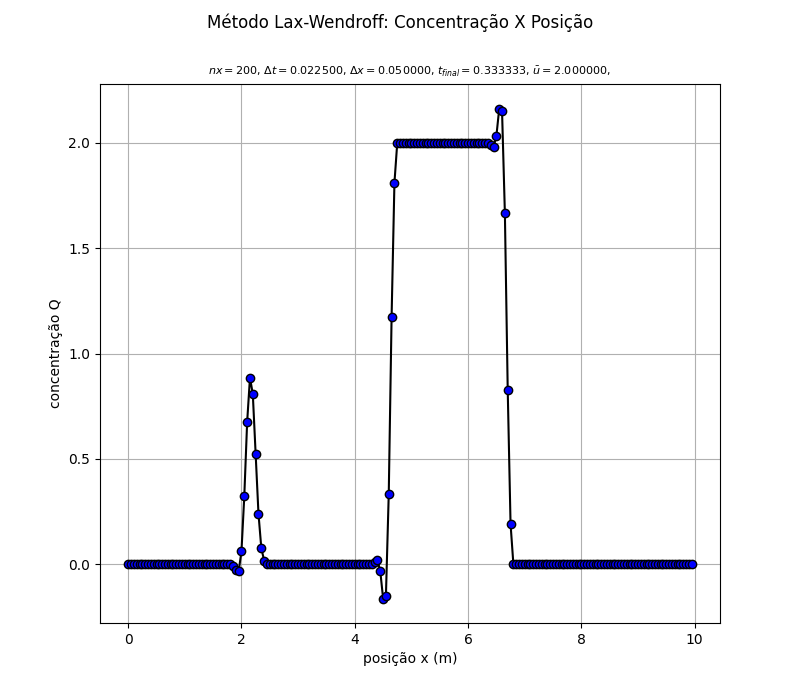
\includegraphics[width=0.7\textwidth]{LWt_final0,333}
    \caption{L-W: $t_{\text{final}} = \frac{1}{3}$s}
\end{figure}
\begin{figure}[H]
    \centering
    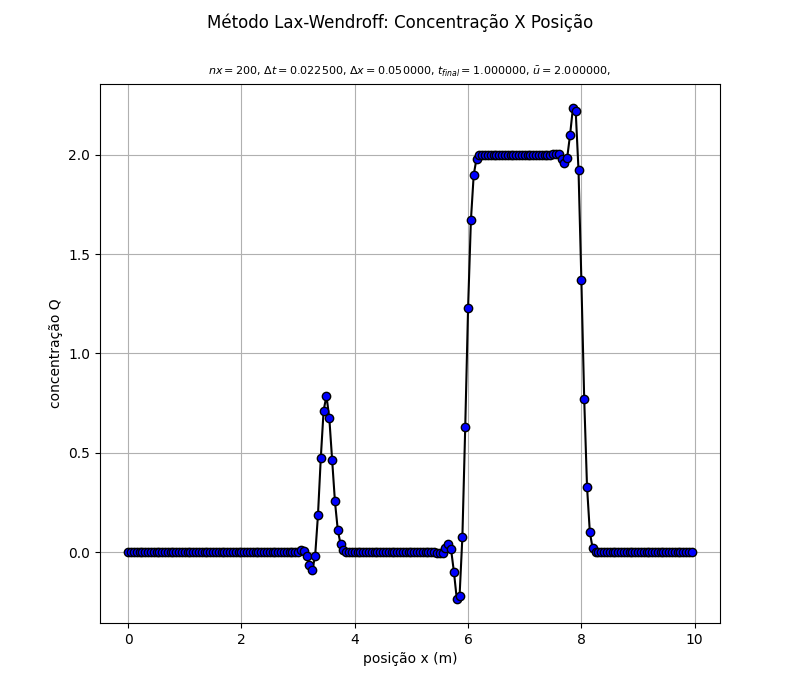
\includegraphics[width=0.7\textwidth]{LWt_final1,0}
    \caption{L-W: $t_{\text{final}} = 1,0$s}
\end{figure}
\begin{figure}[H]
    \centering
    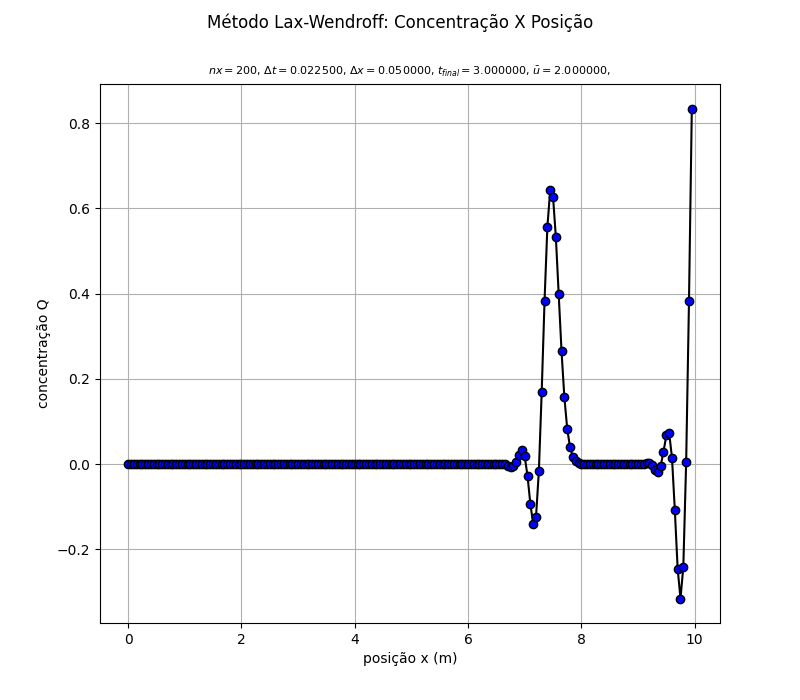
\includegraphics[width=0.7\textwidth]{LWt_final3,0}
    \caption{L-W: $t_{\text{final}} = 3,0$s}
\end{figure}
\begin{figure}[H]
    \centering
    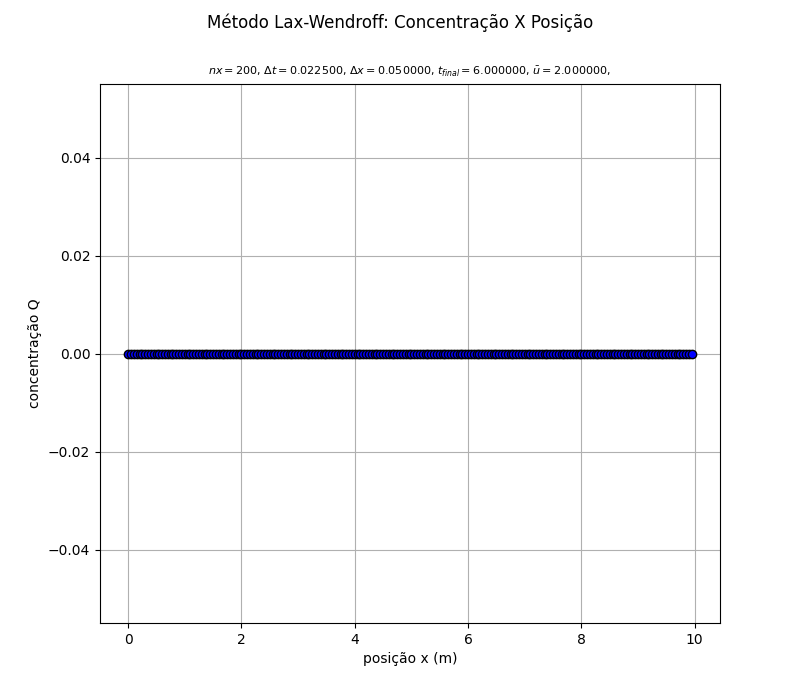
\includegraphics[width=0.7\textwidth]{LWt_final6,0}
    \caption{L-W: $t_{\text{final}} = 6,0$s}
\end{figure}
Nota-se com o avanço do tempo, a onda, representada no gráfico, tende a se
deslocar para a direita, devido ao valor de $\bar{u}$ positivo. Para um tempo
grande o suficiente, a concentração se estabiliza em zero.

\section{Beam-Warming (B-W)}

\subsection{Resultados para variações de $nx$}
Com a variação de $nx$, obtiveram-se os seguintes resultados:
\begin{figure}[H]
    \centering
    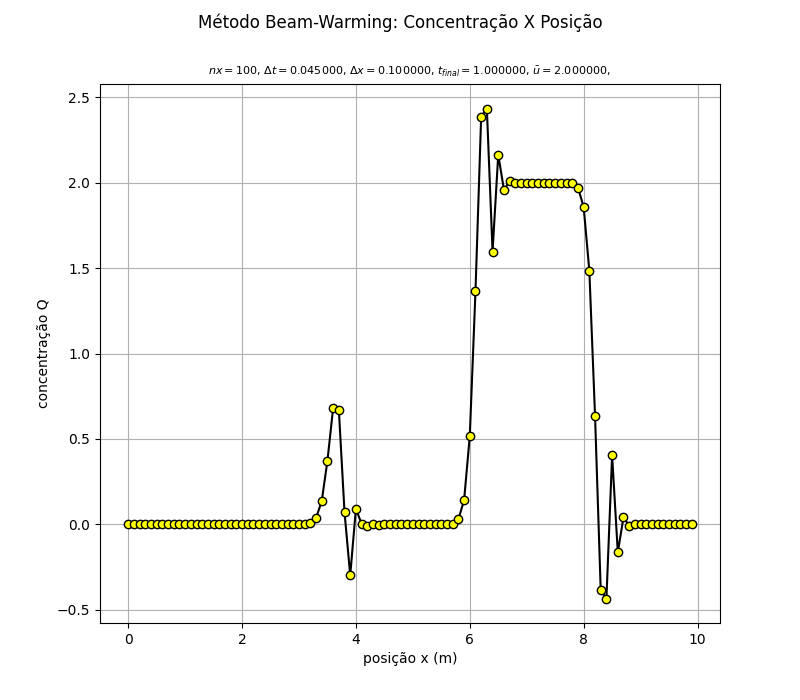
\includegraphics[width=0.7\textwidth]{BWnx100}
    \caption{B-W: $nx = 100$}
\end{figure}
\begin{figure}[H]
    \centering
    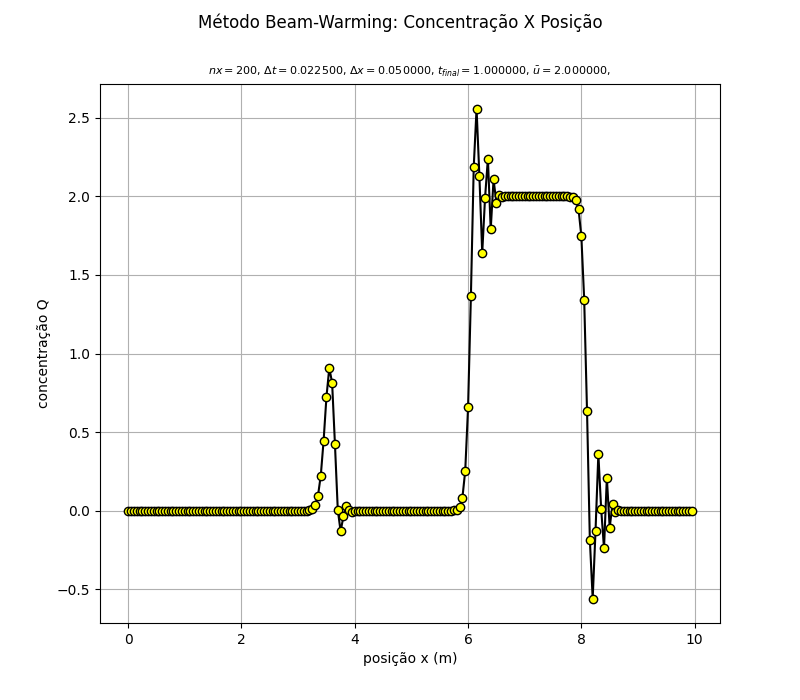
\includegraphics[width=0.7\textwidth]{BWnx200}
    \caption{B-W: $nx = 200$}
\end{figure}
\begin{figure}[H]
    \centering
    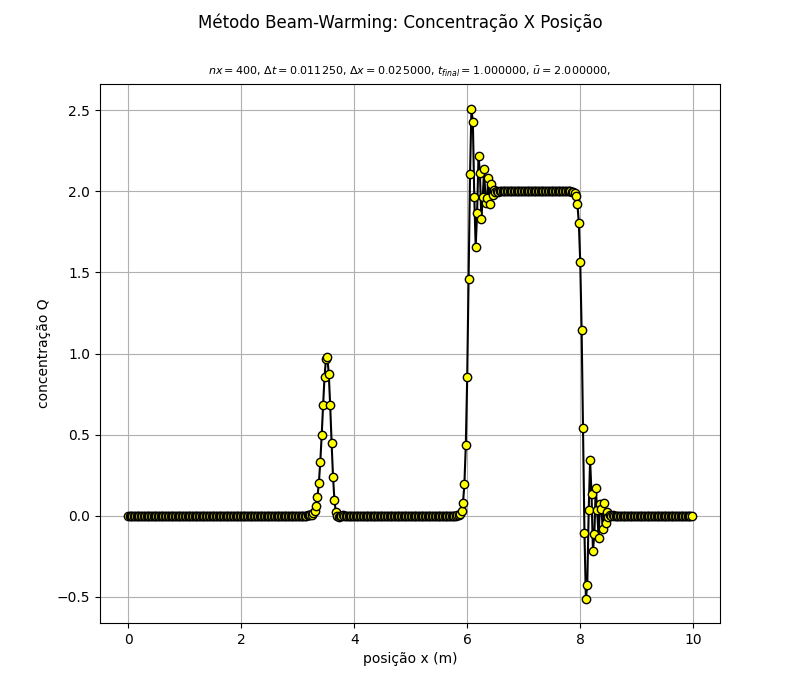
\includegraphics[width=0.7\textwidth]{BWnx400}
    \caption{B-W: $nx = 400$}
\end{figure}
Nota-se que o refinamento da malha resulta em uma curva mais suave, devido ao
aumento da resolução, além disso, nota-se a presença de oscilações numéricas
características do método.

\subsection{Resultados para variações de $t_{\text{final}}$}
Com a variação de $t_{\text{final}}$, obtiveram-se os seguintes resultados:
\begin{figure}[H]
    \centering
    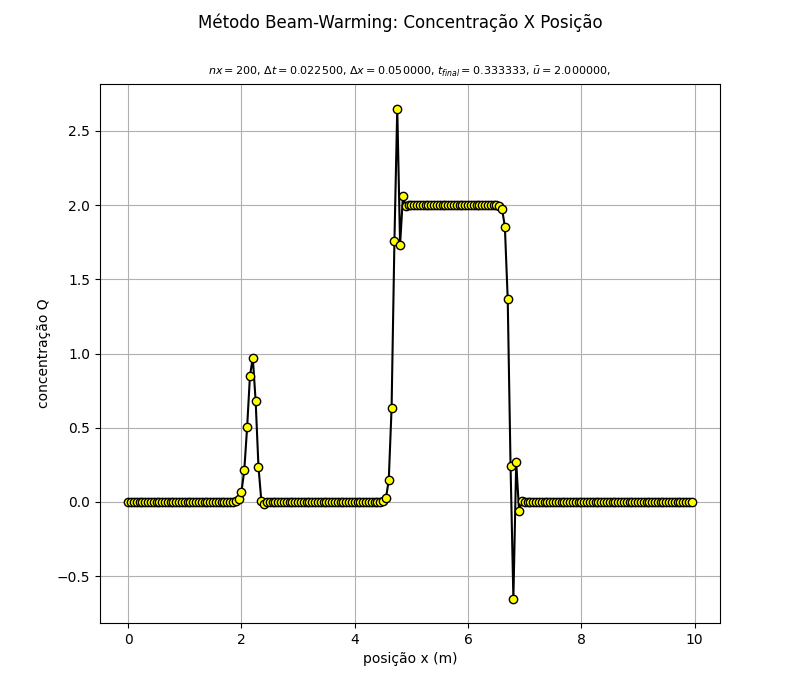
\includegraphics[width=0.7\textwidth]{BWt_final0,333}
    \caption{B-W: $t_{\text{final}} = \frac{1}{3}$s}
\end{figure}
\begin{figure}[H]
    \centering
    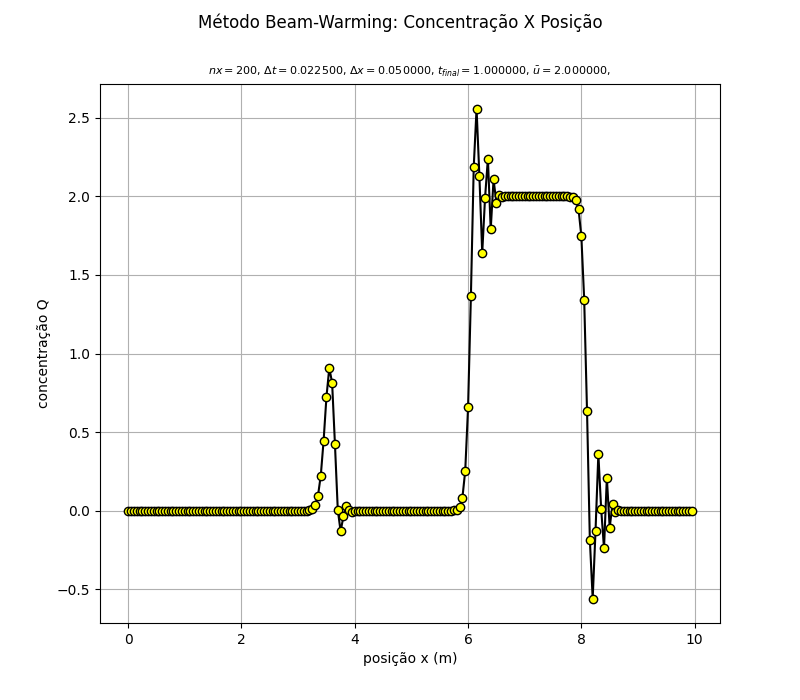
\includegraphics[width=0.7\textwidth]{BWt_final1,0}
    \caption{B-W: $t_{\text{final}} = 1,0$s}
\end{figure}
\begin{figure}[H]
    \centering
    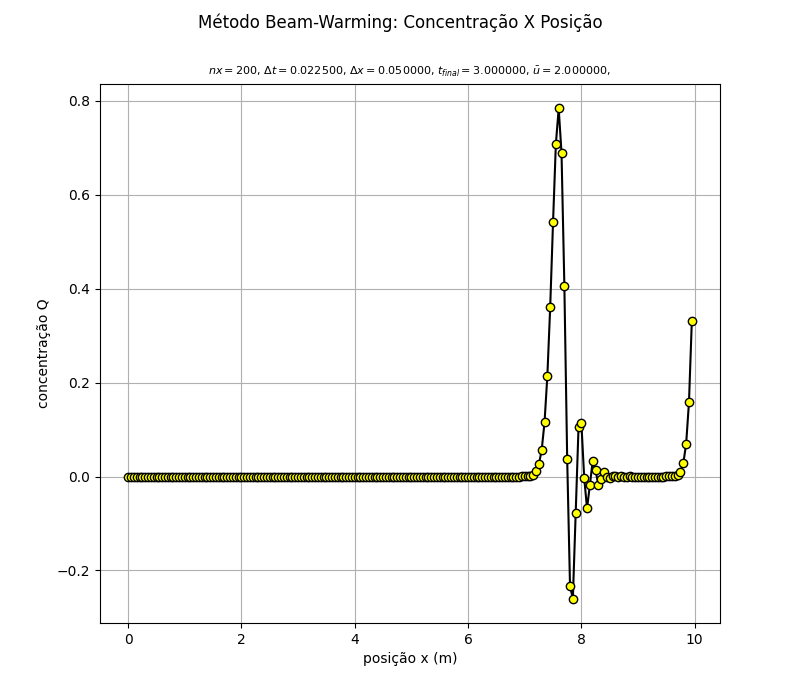
\includegraphics[width=0.7\textwidth]{BWt_final3,0}
    \caption{B-W: $t_{\text{final}} = 3,0$s}
\end{figure}
\begin{figure}[H]
    \centering
    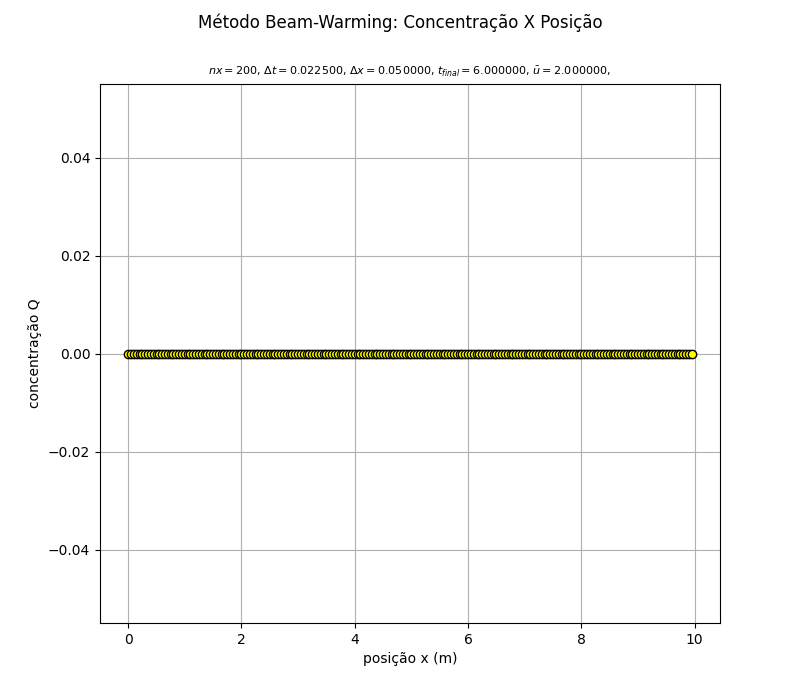
\includegraphics[width=0.7\textwidth]{BWt_final6,0}
    \caption{B-W: $t_{\text{final}} = 6,0$s}
\end{figure}
Nota-se com o avanço do tempo, a onda, representada no gráfico, tende a se
deslocar para a direita, devido ao valor de $\bar{u}$ positivo. Para um tempo
grande o suficiente, a concentração se estabiliza em zero.